\documentclass[xcolor=dvipsnames]{beamer}

\usetheme{Berkeley}

\usepackage{inputenc}
\usepackage{graphicx}
\usepackage{amsmath}
\usepackage{amsthm}

\usepackage{subcaption}
\usepackage{multicol}

\setbeamertemplate{footline}[frame number]

\title{COMP 513 Project}
\subtitle{\textbf{Rolis}}
\date{December 5th 2023}

\author{Presented by \\ Olivier Michaud, Akshay Gopalakrishnan \\ McGill University}


\begin{document}

    \begin{frame}

        \maketitle

    \end{frame}

    \section{Introduction}

    \begin{frame}{Project Description}


        \begin{center}
            Rolis: A software approach to efficiently replicating multi-core transactions 
        \end{center}


        \begin{itemize}
            \item Proposes a new consensus algorithm to improve throughput. 
            \item Uses multiple threads per leader/follower to process transactions. 
            \item Performs well upon failure recovery using \textit{watermarks} to ensure synchronization when necessary.
        \end{itemize}

    \end{frame}

    \begin{frame}{Choice of Experiments}

        \begin{itemize}
            \item Throughput
            \begin{itemize}
                \item vs Silo - Algorithm is built by modifying Silo.  
                \item vs Calvin - Existing state-of-the-art. 
            \end{itemize}    
            \item Latency
            \begin{itemize}
                \item On different batch sizes.  
                \item Measured for $10^{th}, 50^{th}, 95^{th}$ percentiles.
            \end{itemize}         
        \end{itemize}
        
    \end{frame}

    

    \section{Setup}

    
    \begin{frame}{Chosen Test Environment}

        Comparison (right) with original system (left)
        \begin{multicols}{2}
            \begin{itemize}
                \item Azure
                \item 32vCPUs (Intel Xeon Platinum 8272CL) 
                \item 128GB RAM 
                \item 16,000Mbps Network
                \item Ubuntu 18.04 LTS
                \item Hypervisor: Hyper-V
                \item Single Socket (assumed)
                \item AWS EC2
                \item 32vCPUs (Intel Xeon Platinum 8259CL) 
                \item 128GB RAM
                \item 10,000Mbps Network 
                \item Ubuntu Server 20.04 LTS
                \item Hypervisor: KVM based
                \item Shared Instance
            \end{itemize}      
        \end{multicols}
    \end{frame}


    \begin{frame}{Steps to Run}

        \begin{itemize}
            \item Virtual Private Cloud 
            \item Security Groups 
            \item Start EC2 instances.
            \item Setup SSH connections. 
            \item Run $\text{install}.\text{sh}$.
            \item Setup IP addresses (guide given by the paper).
            \item Run $\text{one-click}.\text{sh}$.
        \end{itemize}

    \end{frame}

   
    \section{Experiments}

    \begin{frame}{Throughput: Rolis vs Silo (YCSB++)}
        
        \begin{figure}
            \begin{subfigure}[h]{0.5\textwidth}
                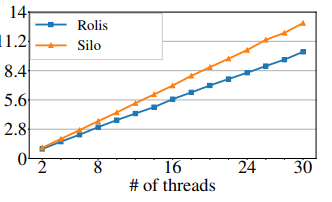
\includegraphics[scale=0.65]{rolis_fig10_ycsb.png}
                \caption{Original}
            \end{subfigure}%
            \hfill
            \begin{subfigure}[h]{0.5\textwidth}
                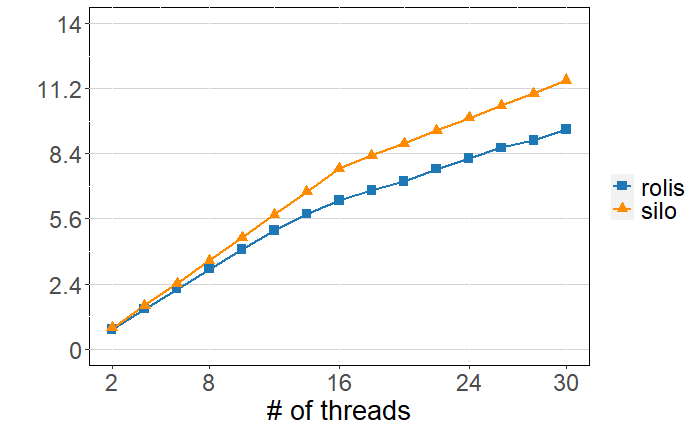
\includegraphics[scale=0.30]{fig10_ycsb.png}
                \caption{Observed}
            \end{subfigure}
        \end{figure}

    \end{frame}

    \begin{frame}{Throughput: Rolis vs Silo (TPC-C)}   
        \begin{figure}
            \begin{subfigure}[h]{0.5\textwidth}
                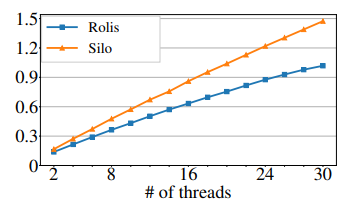
\includegraphics[scale=0.65]{rolis_fig10_tpcc.png}
                \caption{Original}
            \end{subfigure}%
            \hfill
            \begin{subfigure}[h]{0.5\textwidth}
                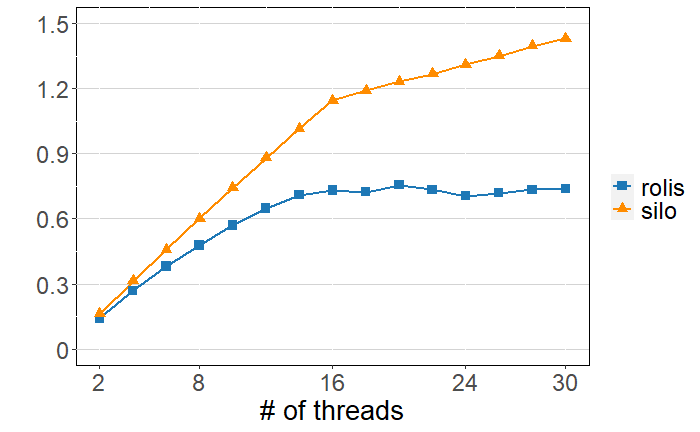
\includegraphics[scale=0.30]{fig10_tpcc.png}
                \caption{Observed}
            \end{subfigure}
        \end{figure}
    \end{frame}

    \begin{frame}{Discuss Observation}

        \begin{figure}
            \begin{subfigure}[h]{0.5\textwidth}
                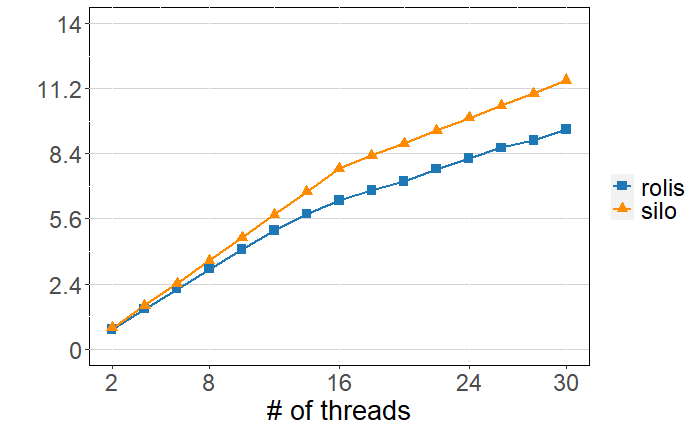
\includegraphics[scale=0.30]{fig10_ycsb.png}
                \caption{YCSB++}
            \end{subfigure}%
            \hfill
            \begin{subfigure}[h]{0.5\textwidth}
                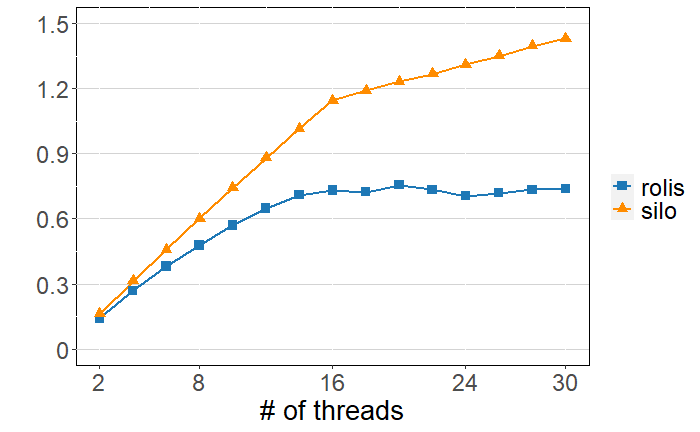
\includegraphics[scale=0.30]{fig10_tpcc.png}
                \caption{TPC-C}
            \end{subfigure}
        \end{figure}

        \begin{itemize}
            \item VM Resource Overcommitment vs Bare Metal Instance. 
            \item CPU sockets.
        \end{itemize}

    \end{frame}

    \begin{frame}{Throughput: Rolis vs Calvin (YCSB++)}
        \begin{figure}
            \begin{subfigure}[h]{0.5\linewidth}
                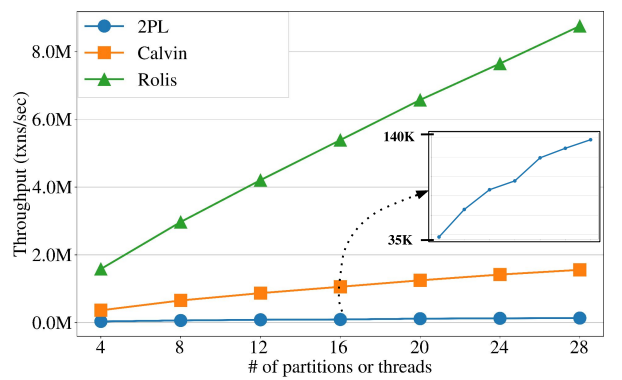
\includegraphics[scale=0.40]{rolis_fig12.png}
                \caption{Original}
            \end{subfigure}%
            \hfill
            \begin{subfigure}[h]{0.5\linewidth}
                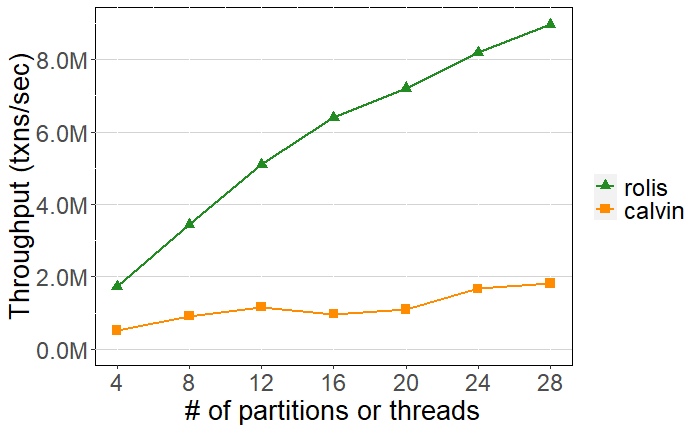
\includegraphics[scale=0.30]{fig12.png}
                \caption{Observed}
            \end{subfigure}           
        \end{figure}
    \end{frame}

    \begin{frame}{Discuss Observation}

        \begin{figure}
            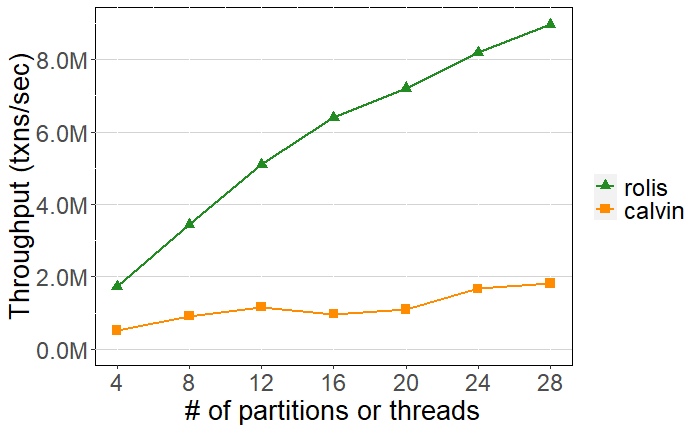
\includegraphics[scale=0.4]{fig12.png}
            \caption{Observed Throughput of Rolis vs Calvin}
        \end{figure}

        \begin{itemize}
            \item Calvin's thread-implementation vs Rolis.
            \item CPU Sockets (Calvin experiment needs just one Machine).
        \end{itemize}


    \end{frame}

    \begin{frame}{Latency: Batch-Size Take 1}
        \begin{figure}
            \begin{subfigure}[h]{0.4\linewidth}
                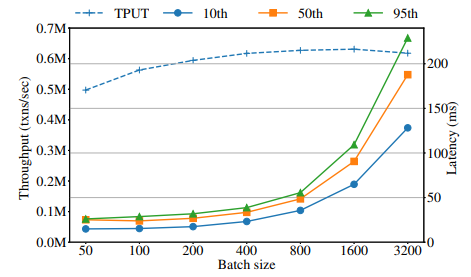
\includegraphics[scale=0.50]{rolis_fig16.png}
                \caption{Original (16 threads)}
            \end{subfigure}
            \hfill
            \begin{subfigure}[h]{0.5\linewidth}
                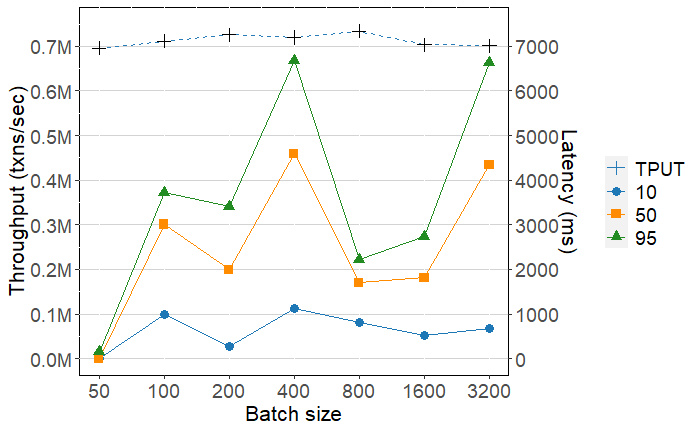
\includegraphics[scale=0.30]{fig16_16t.png}
                \caption{Observed (16 threads)}
            \end{subfigure}
        \end{figure}
    \end{frame}

    \begin{frame}{Latency: Batch-size Take 2}
        \begin{figure}
            \begin{subfigure}[h]{0.4\linewidth}
                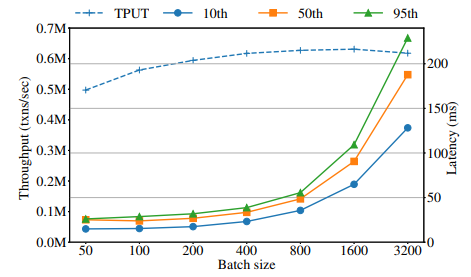
\includegraphics[scale=0.50]{rolis_fig16.png}
                \caption{Original (16 threads)}
            \end{subfigure}
            \hfill
            \begin{subfigure}[h]{0.5\linewidth}
                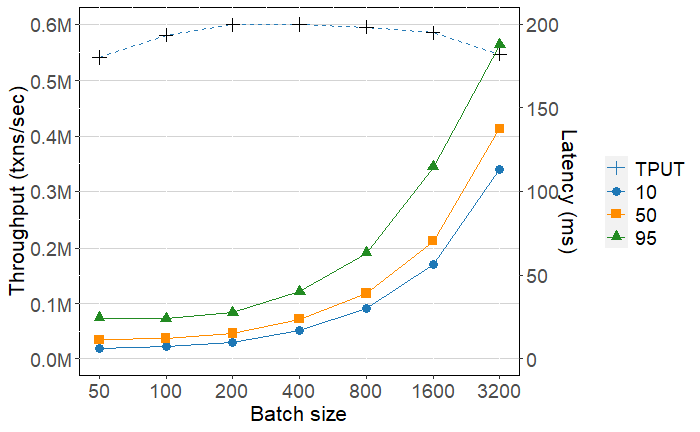
\includegraphics[scale=0.30]{fig16_12t.png}
                \caption{Observed (12 threads)}
            \end{subfigure}
        \end{figure}
    \end{frame}


    \begin{frame}{Discuss Observation}
    
        \begin{figure}
            \begin{subfigure}[h]{0.4\linewidth}
                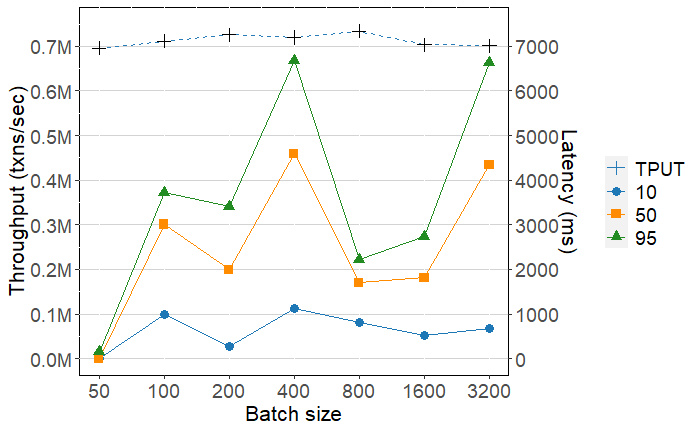
\includegraphics[scale=0.28]{fig16_16t.png}
                \caption{Original (16 threads)}
            \end{subfigure}
            \hfill
            \begin{subfigure}[h]{0.5\linewidth}
                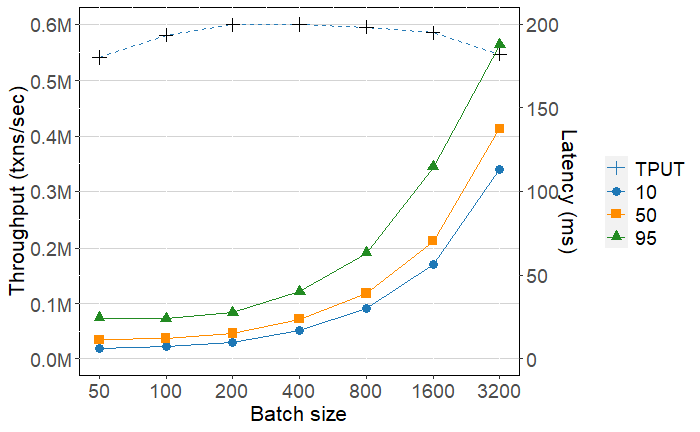
\includegraphics[scale=0.28]{fig16_12t.png}
                \caption{Observed (12 threads)}
            \end{subfigure}
        \end{figure}

        \begin{itemize}
            \item Shared Instances - Network Bandwidth.
            \item Shared Instances - Congestion Control.
        \end{itemize}

    \end{frame}


    \section{Conclusion}

    \begin{frame}{Thank you}

        \begin{itemize}
            \item Rolis: \href{https://dl.acm.org/doi/10.1145/3492321.3519561}{Paper}
            \item Rolis: \href{https://github.com/stonysystems/rolis}{Experiments Repository}
        \end{itemize}

        Questions? 

    \end{frame}

\end{document}